\documentclass[11pt,a4paper]{article}

\usepackage[T1]{fontenc}
\usepackage[utf8]{inputenc}
\usepackage{lmodern}
\usepackage{microtype}
\usepackage[margin=2.35cm]{geometry}
\usepackage{graphicx}
\usepackage{booktabs}
\usepackage{tabularx}
\usepackage{longtable}
\usepackage{array}
\usepackage[table]{xcolor}
\usepackage{hyperref}
\usepackage{listings}
\usepackage{tikz}
\usepackage{pgfplots}
\usepackage{fancyhdr}
\usepackage{enumitem}

\usetikzlibrary{arrows.meta,positioning,shapes.geometric}
\pgfplotsset{compat=1.18}

\definecolor{navy}{HTML}{17365D}
\definecolor{blue}{HTML}{2F75B5}
\definecolor{lightblue}{HTML}{D9EAF7}
\definecolor{lightgray}{HTML}{F2F4F7}
\definecolor{green}{HTML}{548235}
\definecolor{red}{HTML}{C00000}
\definecolor{codebg}{HTML}{F7F8FA}

\hypersetup{
  colorlinks=true,
  linkcolor=navy,
  urlcolor=blue,
  pdftitle={Laporan Hands-on 2: Eksperimen End-to-End MLflow dan Scikit-learn},
  pdfauthor={Nobel Nizam}
}

\pagestyle{fancy}
\fancyhf{}
\lhead{Hands-on 2 MLOps}
\rhead{Nobel Nizam --- 123450117}
\cfoot{\thepage}
\setlength{\headheight}{14pt}

\setlist[itemize]{leftmargin=1.5em,itemsep=2pt,topsep=4pt}
\setlist[enumerate]{leftmargin=1.7em,itemsep=3pt,topsep=4pt}
\renewcommand{\arraystretch}{1.18}

\lstdefinestyle{terminal}{
  backgroundcolor=\color{codebg},
  basicstyle=\ttfamily\small,
  frame=single,
  rulecolor=\color{lightblue},
  breaklines=true,
  columns=fullflexible,
  keepspaces=true,
  showstringspaces=false
}

\newcommand{\stage}[1]{\textcolor{navy}{\textbf{#1}}}
\newcommand{\resultbox}[1]{%
  \begin{center}
    \colorbox{lightblue}{\parbox{0.91\linewidth}{\textbf{Hasil.} #1}}
  \end{center}
}

\begin{document}

\begin{center}
  {\LARGE\bfseries\color{navy} Laporan Hands-on 2}\par
  \vspace{3pt}
  {\large Eksperimen End-to-End MLflow dan Scikit-learn}\par
  \vspace{10pt}
  \begin{tabular}{rl}
    \textbf{Nama} & Nobel Nizam \\
    \textbf{NIM}  & 123450117 \\
    \textbf{Tanggal} & 11 Oktober 2026
  \end{tabular}
\end{center}

\vspace{8pt}
\hrule
\vspace{8pt}

\begin{abstract}
Praktik ini membangun alur eksperimen klasifikasi tumor ganas dari persiapan data hingga rancangan pemuatan model produksi. Dataset Breast Cancer Wisconsin dibagi secara tetap, kemudian delapan konfigurasi baseline dan kandidat dibandingkan menggunakan 5-fold stratified cross-validation. SVC selanjutnya dituning pada 12 kombinasi parameter. Konfigurasi terbaik, yaitu $C=10$ dan $\gamma=\texttt{scale}$, memperoleh recall CV $0{,}965 \pm 0{,}029$ dengan precision $0{,}971 \pm 0{,}018$. Pada test set yang hanya digunakan sekali, model menghasilkan recall 0,929, precision 1,000, F1 0,963, dan ROC-AUC 0,993. Implementasi juga mencakup pencatatan MLflow, nested runs, aturan seleksi otomatis, Model Registry, quality gate, alias \texttt{champion}, DVC, dan audit lineage.
\end{abstract}

\tableofcontents

\section{Pendahuluan}

Eksperimen machine learning tidak hanya menghasilkan sebuah model, tetapi juga melibatkan data, parameter, kode, lingkungan, metrik, dan artefak. Tanpa pencatatan yang konsisten, model terbaik sulit ditelusuri dan hasilnya sulit direproduksi. Hands-on 2 menerapkan alur end-to-end agar setiap keputusan model mempunyai dasar metrik dan lineage yang jelas.

Kasus yang digunakan adalah deteksi tumor ganas pada dataset Breast Cancer Wisconsin. Target asli dibalik sehingga kelas positif bernilai 1 untuk \emph{malignant}. Kesalahan false negative dianggap lebih berbahaya karena tumor ganas dapat terlewat. Oleh sebab itu, recall menjadi \emph{optimizing metric}, sedangkan precision minimal 0,90 menjadi \emph{satisficing metric} agar alarm palsu tetap terkendali.

\subsection{Hipotesis eksperimen}

\begin{enumerate}
  \item \textbf{H1:} model linear sederhana memberikan recall yang jauh lebih baik daripada baseline Dummy.
  \item \textbf{H2:} standardisasi fitur meningkatkan recall model yang sensitif terhadap skala.
  \item \textbf{H3:} tuning SVC meningkatkan recall tanpa menurunkan precision di bawah 0,90.
\end{enumerate}

\section{Lingkungan dan Rancangan Eksperimen}

Eksperimen model dijalankan menggunakan Python 3.13.13, scikit-learn 1.9.0, pandas 3.0.5, dan NumPy 2.5.1. Semua model memakai split data dan fold cross-validation yang sama. Random seed ditetapkan ke 42 untuk mengurangi variasi yang tidak berasal dari model.

\begin{table}[ht]
\centering
\caption{Keputusan eksperimen sebelum training.}
\begin{tabularx}{\linewidth}{>{\bfseries}p{0.28\linewidth}X}
\toprule
Aspek & Keputusan \\
\midrule
Dataset & \texttt{sklearn.datasets.load\_breast\_cancer}, 569 sampel dan 30 fitur numerik \\
Kelas positif & 1 = malignant setelah target asli dibalik \\
Split & 80\% train dan 20\% test, stratified, seed 42 \\
Seleksi model & 5-fold Stratified CV pada train set \\
Optimizing metric & Recall \\
Satisficing metric & Precision $\geq 0{,}90$ \\
Test set & Digunakan sekali setelah kandidat dipilih \\
\bottomrule
\end{tabularx}
\end{table}

\subsection{Alur kerja}

\begin{center}
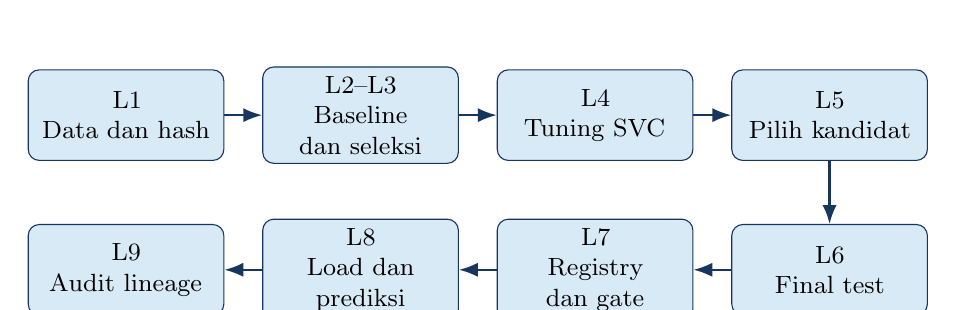
\begin{tikzpicture}[
  node distance=0.48cm,
  box/.style={draw=navy, rounded corners, fill=lightblue, minimum height=1.15cm,
              text width=2.25cm, align=center, font=\small},
  arrow/.style={-{Latex[length=2.4mm]}, thick, draw=navy}
]
  \node[box] (l1) {L1\\Data dan hash};
  \node[box, right=of l1] (l23) {L2--L3\\Baseline dan seleksi};
  \node[box, right=of l23] (l4) {L4\\Tuning SVC};
  \node[box, right=of l4] (l5) {L5\\Pilih kandidat};
  \node[box, below=0.8cm of l5] (l6) {L6\\Final test};
  \node[box, left=of l6] (l7) {L7\\Registry dan gate};
  \node[box, left=of l7] (l8) {L8\\Load dan prediksi};
  \node[box, left=of l8] (l9) {L9\\Audit lineage};
  \draw[arrow] (l1) -- (l23);
  \draw[arrow] (l23) -- (l4);
  \draw[arrow] (l4) -- (l5);
  \draw[arrow] (l5) -- (l6);
  \draw[arrow] (l6) -- (l7);
  \draw[arrow] (l7) -- (l8);
  \draw[arrow] (l8) -- (l9);
\end{tikzpicture}
\end{center}

Kode dipisahkan berdasarkan tanggung jawab: \texttt{data.py} menangani data, \texttt{tracking.py} menyeragamkan logging, \texttt{train.py} menjalankan eksperimen, \texttt{evaluate.py} memilih dan menguji kandidat, sedangkan \texttt{register.py}, \texttt{predict.py}, dan \texttt{reproduce.py} menangani siklus model setelah training.

\section{Pelaksanaan dan Hasil}

\subsection{L1 --- Persiapan, Split, dan Versi Data}

Dataset dimuat sebagai DataFrame, target dibalik, lalu dibagi secara stratified. Train set disimpan sebagai \texttt{data/train.csv} dan test set sebagai \texttt{data/test.csv}. Sidik jari dataset dihitung dari seluruh nilai dan indeks menggunakan MD5. Pipeline DVC didefinisikan pada \texttt{dvc.yaml}; file CSV diabaikan Git sehingga versi data direpresentasikan oleh metadata DVC.

\begin{lstlisting}[style=terminal]
python -m src.data --force
# Train: 455 baris
# Test : 114 baris
# Data MD5: ee5481ad12c0896439e993aacc9e8d50
\end{lstlisting}

\begin{table}[ht]
\centering
\caption{Distribusi kelas setelah split.}
\begin{tabular}{lrrr}
\toprule
Subset & Benign (0) & Malignant (1) & Total \\
\midrule
Train & 285 & 170 & 455 \\
Test  & 72  & 42  & 114 \\
\bottomrule
\end{tabular}
\end{table}

\resultbox{Split menghasilkan proporsi kelas yang hampir sama pada kedua subset. Hash yang tetap memberikan identitas data yang dapat dicatat pada setiap run dan diperiksa kembali saat reproduksi.}

\subsection{L2 --- Baseline dan Controlled Experiment}

Baseline Dummy selalu memprediksi kelas mayoritas. Dua Logistic Regression kemudian dibandingkan dengan satu perubahan saja, yaitu penggunaan \texttt{StandardScaler}. Semua model menggunakan data dan fold yang sama.

\begin{table}[ht]
\centering
\caption{Hasil baseline (rata-rata $\pm$ simpangan baku CV).}
\begin{tabular}{lccc}
\toprule
Model & Recall & Precision & F1 \\
\midrule
Dummy & $0{,}000 \pm 0{,}000$ & $0{,}000 \pm 0{,}000$ & $0{,}000 \pm 0{,}000$ \\
LogReg tanpa scaling & $0{,}918 \pm 0{,}034$ & $0{,}958 \pm 0{,}024$ & $0{,}937 \pm 0{,}018$ \\
LogReg + scaling & $0{,}953 \pm 0{,}040$ & $0{,}977 \pm 0{,}028$ & $0{,}964 \pm 0{,}021$ \\
\bottomrule
\end{tabular}
\end{table}

\resultbox{Dummy gagal mendeteksi seluruh tumor ganas. Logistic Regression tanpa scaling langsung mencapai recall 0,918. Standardisasi menaikkan recall sekitar 0,035 dan sekaligus meningkatkan precision serta F1. H1 dan H2 mendapat dukungan awal.}

\subsection{L3 --- Perbandingan Kandidat Model}

Lima algoritma tambahan dibandingkan: KNN, Decision Tree, Random Forest, Gradient Boosting, dan SVC. Preprocessing serta fold CV dibuat identik agar perbedaan metrik terutama berasal dari algoritma.

\begin{table}[ht]
\centering
\small
\caption{Ringkasan seluruh hasil model sebelum tuning.}
\begin{tabular}{lcccc}
\toprule
Model & Recall & Precision & F1 & ROC-AUC \\
\midrule
Dummy & $0{,}000 \pm 0{,}000$ & $0{,}000 \pm 0{,}000$ & $0{,}000 \pm 0{,}000$ & $0{,}500 \pm 0{,}000$ \\
LogReg tanpa scaling & $0{,}918 \pm 0{,}034$ & $0{,}958 \pm 0{,}024$ & $0{,}937 \pm 0{,}018$ & $0{,}993 \pm 0{,}006$ \\
LogReg + scaling & $0{,}953 \pm 0{,}040$ & $0{,}977 \pm 0{,}028$ & $0{,}964 \pm 0{,}021$ & $0{,}996 \pm 0{,}005$ \\
KNN & $0{,}918 \pm 0{,}034$ & $0{,}988 \pm 0{,}025$ & $0{,}951 \pm 0{,}026$ & $0{,}987 \pm 0{,}014$ \\
Decision Tree & $0{,}853 \pm 0{,}085$ & $0{,}894 \pm 0{,}037$ & $0{,}872 \pm 0{,}057$ & $0{,}887 \pm 0{,}061$ \\
Random Forest & $0{,}935 \pm 0{,}039$ & $0{,}964 \pm 0{,}011$ & $0{,}949 \pm 0{,}021$ & $0{,}989 \pm 0{,}007$ \\
Gradient Boosting & $0{,}947 \pm 0{,}034$ & $0{,}965 \pm 0{,}021$ & $0{,}955 \pm 0{,}020$ & $0{,}991 \pm 0{,}005$ \\
SVC default & $0{,}947 \pm 0{,}034$ & $0{,}977 \pm 0{,}021$ & $0{,}961 \pm 0{,}008$ & $0{,}995 \pm 0{,}005$ \\
\bottomrule
\end{tabular}
\end{table}

Decision Tree menjadi satu-satunya model non-Dummy yang tidak memenuhi precision 0,90. Logistic Regression dengan scaling menghasilkan recall tertinggi sebelum tuning, sedangkan SVC mempunyai kombinasi recall, precision, F1, dan ROC-AUC yang kuat sehingga layak dituning.

\begin{center}
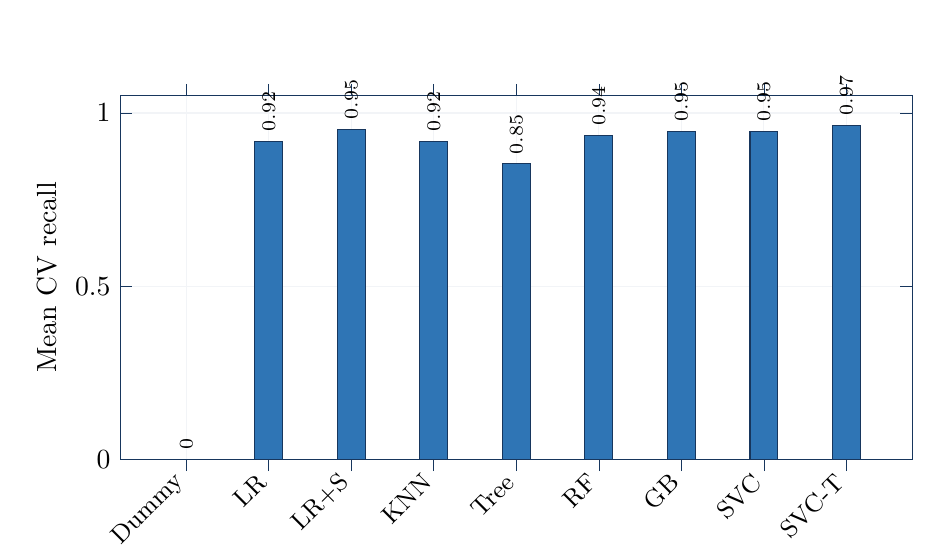
\begin{tikzpicture}
\begin{axis}[
  ybar,
  width=0.96\linewidth,
  height=6.2cm,
  ymin=0,ymax=1.05,
  ylabel={Mean CV recall},
  symbolic x coords={Dummy,LR,LR+S,KNN,Tree,RF,GB,SVC,SVC-T},
  xtick=data,
  x tick label style={rotate=45,anchor=east,font=\small},
  bar width=10pt,
  nodes near coords,
  nodes near coords style={font=\scriptsize,rotate=90,anchor=west},
  grid=major,
  grid style={draw=lightgray},
  axis line style={draw=navy},
  tick style={draw=navy}
]
\addplot[fill=blue,draw=navy] coordinates {
  (Dummy,0.000) (LR,0.918) (LR+S,0.953) (KNN,0.918) (Tree,0.853)
  (RF,0.935) (GB,0.947) (SVC,0.947) (SVC-T,0.965)
};
\end{axis}
\end{tikzpicture}
\end{center}

\subsection{L4 --- Hyperparameter Tuning dengan Nested Runs}

SVC RBF dituning memakai \texttt{GridSearchCV}. Ruang pencarian berisi empat nilai $C$ dan tiga nilai $\gamma$, sehingga terdapat 12 kombinasi. Implementasi MLflow membuat satu parent run \texttt{10-svc-gridsearch}; setiap kombinasi dicatat sebagai child run beserta parameter, mean, dan standard deviation seluruh metrik.

\begin{table}[ht]
\centering
\caption{Konfigurasi dan hasil terbaik tuning SVC.}
\begin{tabular}{ll}
\toprule
Komponen & Hasil \\
\midrule
Ruang $C$ & 0,1; 1; 10; 100 \\
Ruang $\gamma$ & \texttt{scale}; 0,01; 0,001 \\
Jumlah kombinasi & 12 \\
Parameter terbaik & $C=10$, $\gamma=\texttt{scale}$ \\
CV recall & $0{,}965 \pm 0{,}029$ \\
CV precision & $0{,}971 \pm 0{,}018$ \\
CV F1 & $0{,}967 \pm 0{,}011$ \\
CV ROC-AUC & $0{,}993 \pm 0{,}006$ \\
\bottomrule
\end{tabular}
\end{table}

\resultbox{Tuning meningkatkan point estimate recall SVC dari 0,947 menjadi 0,965 tanpa melanggar precision minimum. Kenaikan 0,018 masih lebih kecil daripada simpangan baku recall antarfold, sehingga hasil ini belum cukup untuk klaim peningkatan yang kuat secara statistik.}

\subsection{L5 --- Seleksi Kandidat secara Programatik}

Run kandidat difilter dengan aturan \texttt{cv\_precision\_mean >= 0.90}, lalu diurutkan berdasarkan recall dan F1. Aturan ini menghindari pemilihan manual berdasarkan perasaan atau hanya satu metrik. Dengan hasil yang diperoleh, parent run SVC hasil tuning menjadi kandidat utama karena recall CV tertinggi dan precision 0,971.

\resultbox{Kandidat terpilih adalah SVC dengan $C=10$ dan $\gamma=\texttt{scale}$. Decision Tree otomatis tersaring karena precision rata-ratanya hanya 0,894.}

\subsection{L6 --- Evaluasi Final pada Test Set}

Model kandidat dilatih ulang pada seluruh train set, kemudian test set digunakan satu kali. Skrip \texttt{evaluate.py} menolak evaluasi ulang bila run sudah memiliki tag \texttt{test\_evaluated=true}. Metrik test ditambahkan pada run kandidat yang sama agar lineage tidak terputus.

\begin{table}[ht]
\centering
\caption{Hasil final test set untuk SVC hasil tuning.}
\begin{tabular}{lr}
\toprule
Metrik & Nilai \\
\midrule
Recall & 0,9286 \\
Precision & 1,0000 \\
F1 & 0,9630 \\
ROC-AUC & 0,9927 \\
\bottomrule
\end{tabular}
\hspace{1.5cm}
\begin{tabular}{c|cc}
\multicolumn{3}{c}{\textbf{Confusion matrix}} \\
 & Pred. benign & Pred. malignant \\
\hline
Aktual benign & 72 & 0 \\
Aktual malignant & 3 & 39 \\
\end{tabular}
\end{table}

\resultbox{Tidak terdapat false positive, tetapi tiga dari 42 tumor ganas terlewat. Recall test turun sekitar 0,036 dari mean CV, sedangkan precision tetap sempurna. Model masih memenuhi quality gate precision.}

\subsection{L7 --- Model Registry dan Quality Gate}

Skrip \texttt{register.py} mendaftarkan URI kandidat sebagai versi baru pada registry model. Setelah itu, skrip menambahkan alias \texttt{challenger} dan membandingkannya dengan champion. Promosi dilakukan jika test precision minimal 0,90 dan test recall setidaknya 0,005 di atas champion. Hash data champion dan challenger juga harus sama agar perbandingan adil.

\begin{lstlisting}[style=terminal]
passed = (test_precision >= 0.90 and
          test_recall >= champion_recall + 0.005)
\end{lstlisting}

Aturan quality gate telah diuji dengan unit test untuk kondisi lolos, precision terlalu rendah, dan peningkatan recall yang belum cukup. Pada registry kosong, kandidat pertama dengan precision 1,000 memenuhi syarat menjadi champion awal.

\subsection{L8 --- Pemuatan Model dan Prediksi}

Aplikasi tidak menggunakan path file atau nomor versi yang ditulis langsung. Skrip \texttt{predict.py} memuat model melalui URI berikut:

\begin{lstlisting}[style=terminal]
models:/bc-malignant-classifier@champion
\end{lstlisting}

Pendekatan alias memisahkan kode aplikasi dari versi model. Ketika champion berubah, kode prediksi tetap sama; service hanya perlu memuat ulang model. Signature yang disimpan bersama model membantu memeriksa struktur dan tipe input.

\subsection{L9 --- Reproducibility dan Audit Lineage}

Skrip \texttt{reproduce.py} menelusuri alias champion menuju model version dan run sumber. Run tersebut menyediakan nama run, parameter, metrik, hash data, serta commit Git. Hash data saat ini dibandingkan dengan tag \texttt{data\_md5}; ketidaksesuaian menghentikan proses karena hasil tidak lagi dapat dianggap reproduksi dari eksperimen yang sama.

\begin{lstlisting}[style=terminal]
Prediksi -> @champion -> model version -> run
          -> parameter, metrik, commit Git, data MD5, artifact
\end{lstlisting}

Commit implementasi yang menjadi dasar eksperimen adalah \texttt{98bc3e1}, sedangkan hash dataset adalah \texttt{ee5481ad12c0896439e993aacc9e8d50}.

\section{Validasi Implementasi dan Keterbatasan}

Validasi yang berhasil dilakukan mencakup kompilasi seluruh modul Python, empat unit test untuk split, hash, dan quality gate, serta eksekusi scikit-learn terhadap baseline, seluruh kandidat, 12 kombinasi tuning, dan final test. Angka hasil pada laporan berasal dari eksekusi tersebut.

\begin{table}[ht]
\centering
\caption{Status validasi praktik.}
\begin{tabularx}{\linewidth}{>{\bfseries\raggedright\arraybackslash}p{0.35\linewidth}>{\raggedright\arraybackslash}p{0.16\linewidth}>{\raggedright\arraybackslash}X}
\toprule
Komponen & Status & Keterangan \\
\midrule
Split, hash, dan CSV & Berhasil & Data train/test dibuat dan hash stabil \\
Baseline serta model selection & Berhasil & Delapan konfigurasi dieksekusi dengan 5-fold CV \\
GridSearchCV & Berhasil & Seluruh 12 kombinasi selesai \\
Final test & Berhasil & Metrik dan confusion matrix dihitung \\
Unit test dan compile check & Berhasil & Empat unit test lulus; modul dapat dikompilasi \\
MLflow server dan UI & Belum dijalankan & Paket MLflow tidak tersedia dan instalasi jaringan diblokir \\
DVC runtime & Belum dijalankan & Metadata DVC tersedia, tetapi paket DVC tidak tersedia \\
Registry, alias, dan serving & Belum dijalankan & Kode tersedia; memerlukan server MLflow aktif \\
\bottomrule
\end{tabularx}
\end{table}

Keterbatasan tersebut berarti laporan tidak mengklaim adanya run, screenshot MLflow UI, model version, atau alias yang benar-benar tersimpan pada server. Setelah dependensi dapat dipasang, alur yang sama dapat dijalankan melalui \texttt{run\_pipeline.sh} untuk menghasilkan artefak tracking dan registry.

\section{Analisis Hipotesis}

\begin{enumerate}
  \item \textbf{H1 didukung.} Recall meningkat dari 0,000 pada Dummy menjadi 0,918 pada Logistic Regression tanpa scaling. Baseline Dummy menunjukkan bahwa accuracy kelas mayoritas tidak cukup untuk kasus medis yang berfokus pada kelas positif.
  \item \textbf{H2 didukung pada eksperimen ini.} StandardScaler menaikkan recall Logistic Regression dari 0,918 menjadi 0,953 dan F1 dari 0,937 menjadi 0,964. Perbandingan terkontrol membuat scaling menjadi satu-satunya perubahan utama.
  \item \textbf{H3 didukung secara point estimate, tetapi belum kuat secara statistik.} Tuning menaikkan recall SVC dari 0,947 menjadi 0,965 dengan precision 0,971. Selisih recall 0,018 masih berada dalam variasi antarfold, sehingga repeated CV atau pengujian statistik diperlukan untuk klaim yang lebih kuat.
\end{enumerate}

Hasil test memperlihatkan trade-off yang sesuai tujuan: tidak ada benign yang salah diberi alarm malignant, tetapi masih ada tiga malignant yang terlewat. Dalam konteks klinis, threshold keputusan dapat ditinjau kembali untuk mengejar recall lebih tinggi, kemudian dampaknya terhadap precision harus diukur pada data validasi yang terpisah.

\section{Kesimpulan}

Hands-on 2 berhasil menunjukkan bahwa eksperimen model yang baik membutuhkan lebih dari sekadar nilai akurasi. Split dan fold yang tetap membuat perbandingan adil; baseline membuktikan manfaat model; scaling meningkatkan model linear; dan tuning SVC menghasilkan kandidat dengan recall CV tertinggi tanpa melanggar precision minimum. Pada test set, model terbaik mencapai recall 0,929, precision 1,000, F1 0,963, dan ROC-AUC 0,993.

Praktik juga memperlihatkan peran MLflow dan DVC dalam rancangan MLOps: parameter, data, metrik, model, dan lineage ditempatkan dalam satu alur; seleksi kandidat serta quality gate dinyatakan sebagai aturan kode; dan aplikasi memuat model melalui alias, bukan versi yang ditulis langsung. Dengan demikian, eksperimen menjadi lebih terukur, dapat diaudit, dan siap dihubungkan ke otomasi CI/CD/CT setelah tracking server serta dependensi tersedia.

\appendix
\section{Perintah Reproduksi}

\begin{lstlisting}[style=terminal]
cd handson-2
python -m venv .venv
source .venv/bin/activate
pip install -r requirements.txt
dvc repro prepare

# Terminal 1
./start_server.sh

# Terminal 2
./run_pipeline.sh
\end{lstlisting}

Tahap juga dapat dijalankan terpisah dalam urutan berikut:

\begin{lstlisting}[style=terminal]
src.data -> src.train -> src.evaluate -> src.register
         -> src.predict -> src.reproduce
\end{lstlisting}

MLflow UI tersedia pada \url{http://127.0.0.1:5000} ketika server aktif.

\end{document}
